%%%%%%%%%%%%%%%%%%%%%%%%%%%%%%%%%%%%%%%%%%%%%%%%%%%%%%%%%%%%%%%%%%%%%%%%%%%%%%%
% Chapter 'Absorption - R-32 - lubricant PEB8'
%%%%%%%%%%%%%%%%%%%%%%%%%%%%%%%%%%%%%%%%%%%%%%%%%%%%%%%%%%%%%%%%%%%%%%%%%%%%%%%
\subsection{Lubricant PEB8}
%
%%%%%%%%%%%%%%%%%%%%%%%%%%%%%%%%%%%%%%%%%%%%%%%%%%%%%%%%%%%%%%%%%%%%%%%%%%%%%%%
%%%%%%%%%%%%%%%%%%%%%%%%%%%%%%%%%%%%%%%%%%%%%%%%%%%%%%%%%%%%%%%%%%%%%%%%%%%%%%%
\subsubsection{FloryHuggins - ID 1}
%
\begin{tabular}[l]{|lp{11.5cm}|}
\hline
\addlinespace

\textbf{Sorbent:} & lubricant \\
\textbf{Subtype:} & PEB8 \\
\textbf{Refrigerant:} & R-32 \\
\textbf{Equation:} & FloryHuggins \\
\textbf{ID:} & 1 \\
\textbf{Reference:} & Wahlström, Åsa; Vamling, Lennart (2000): Solubility of HFCs in Pentaerythritol Tetraalkyl Esters. In: J. Chem. Eng. Data 45 (1), S. 97–103. DOI: 10.1021/je990171n. \\
\textbf{Comment:} & None \\

\addlinespace
\hline
\end{tabular}
\newline

\textbf{Equation and parameters:}
\newline
%
Pressure $p$ in $\si{\pascal}$ is calculated depending on molar fraction of refrigerant in the liquid phase $x_1$ in $\si{\mole\per\mole}$, temperature $T$ in $\si{\kelvin}$, molar volumes of both components ($v_1$ and $v_2$) in $\si{\cubic\meter\per\mole}$, and vapor pressure $p_\mathrm{sat,1}$ in $\si{\pascal}$. If molar volumes less than zero are used as function arguements, constant molar volumes given by parameter record are used. Equilibrium equation is given by:
%
\begin{equation*}
\begin{split}
p &=& \gamma_1 x_1 p_\mathrm{sat,1} & \quad\text{, and} \\
\gamma_1 &=& \exp \left( \ln \left( 1 - \left( 1 - \nicefrac{1}{r} \right) \Phi_2  \right) + \left(1 - \nicefrac{1}{r}\right) \Phi_2 + \Gamma \Phi_2 ^2 \right) & \quad\text{, and} \\
\Phi_2 &=& r \frac{x_2}{x_1 + r x_2} & \quad\text{, and} \\
\Gamma &=& \nicefrac{w_0^{*}}{T} \left( 1 + \nicefrac{w_1}{T} \right) & \quad\text{, and} \\
x_2 &=& 1 - x_1  & \quad\text{.} \\
\end{split}
\end{equation*}
%
The parameters of the equation are:
%
\begin{longtable}[l]{lll|lll}
\toprule
\addlinespace
\textbf{Par.} & \textbf{Unit} & \textbf{Value} &	\textbf{Par.} & \textbf{Unit} & \textbf{Value} \\
\addlinespace
\midrule
\endhead

\bottomrule
\endfoot
\bottomrule
\endlastfoot
\addlinespace

$r$ & - & 1.158000000e+01 & $w_0^{*}$ & $\si{\kelvin}$ & 7.750000000e+02 \\
$w_1$ & $\si{\kelvin}$ & -1.770000000e+02 & & & \\

\addlinespace\end{longtable}

\textbf{Validity:}
\newline
Equation is approximately valid for $303.15 \si{\kelvin} \leq T \leq 363.15 \si{\kelvin}$.
\newline

\textbf{Visualization:}
%
\begin{figure}[!htp]
{\noindent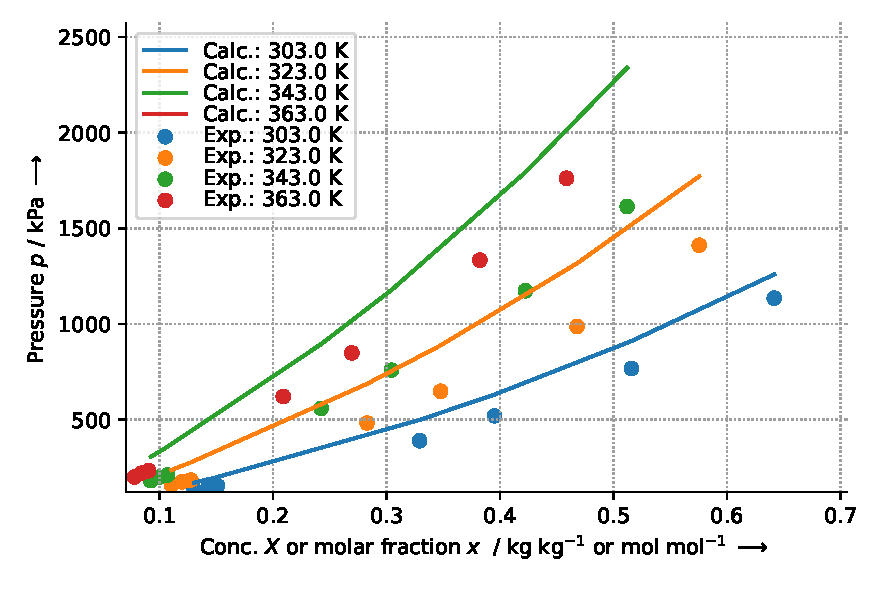
\includegraphics[height=10cm, keepaspectratio]{figs/abs/abs_R-32_lubricant_PEB8_FloryHuggins_1.pdf}}
\end{figure}
%

To generate the figure, the following refrigerant functions were selected:
\begin{itemize}
\item Vapor pressure: VaporPressure\_EoS1 - ID 1
\item Saturated liquid density: SaturatedLiquidDensity\_EoS1 - ID 1
\end{itemize}

The uncertainity of the experimental data is:
\begin{itemize}
\item Data source $\,\to\,$ Data was taken from table
\end{itemize}

The mean absolute percentage error (MAPE) between the experimental and calculated data results in 41.26\%.
\FloatBarrier
\newpage
%%%%%%%%%%%%%%%%%%%%%%%%%%%%%%%%%%%%%%%%%%%%%%%%%%%%%%%%%%%%%%%%%%%%%%%%%%%%%%%
%%%%%%%%%%%%%%%%%%%%%%%%%%%%%%%%%%%%%%%%%%%%%%%%%%%%%%%%%%%%%%%%%%%%%%%%%%%%%%%
\subsubsection{MixingRule - ID 1}
%
\begin{tabular}[l]{|lp{11.5cm}|}
\hline
\addlinespace

\textbf{Sorbent:} & lubricant \\
\textbf{Subtype:} & PEB8 \\
\textbf{Refrigerant:} & R-32 \\
\textbf{Equation:} & MixingRule \\
\textbf{ID:} & 1 \\
\textbf{Reference:} & Yokozeki, A. (2001): Solubility of Refrigerant in Various Lubricants. In: International Journal of Thermophysics 22 (4), S. 1057–1071. DOI: 10.1023/A:1010695705260. \\
\textbf{Comment:} & None \\

\addlinespace
\hline
\end{tabular}
\newline

\textbf{Equation and parameters:}
\newline
%
Vapor pressure $p_\mathrm{sat}$ in $\si{\pascal}$ is calculated depending on temperature $T$ in $\si{\kelvin}$ and molar volume v in $\si{\mole\per\cubic\meter}$ by using cubic equation of state. For this purpose, molar volumes of liquid and vapor phase are changed iteratively until fugacity coefficients of vapor and liquid phase are equal. Cubic equation of state and mixing rules are given by:
\begin{equation*}
\begin{split}
p &=& R \frac{T}{v - b} - \frac{a}{v \left(v + b\right)} & \quad\text{, and} \\
a &=& z_1^2 a_1 + 2 z_1 z_2 a_{12} + 2_2^2 a_2 & \quad\text{, and} \\
b &=& z_1^2 b_1 + 2 z_1 z_2 b_{12} + 2_2^2 b_2 & \quad\text{, and} \\
a_{12} &=& \left( a_1 a_2 \right) ^{0.5} \left( 1 + \nicefrac{t}{T} \right) \left(1 - k_{12} \right) & \quad\text{, and} \\
b_{12} &=& \frac{ b_1 + b_2 }{2} \left(1 - m \right) & \quad\text{, and} \\
k_{12} &=& \frac{l_{12} l_{21} \left(z_1 + z_2 \right)}{l_{21} z_1 + l_{12} z_2} & \quad\text{, and} \\
z_j &=& x_j \textrm { or } y_j \textrm{ depending on phase} & \quad\text{, and} \\
a_j &=& \frac{1}{9 \left(2^{\nicefrac{1}{3}} - 1\right)} \frac{\left(R T_{\mathrm{crit},j} \right)^2}{p_{\mathrm{crit},j}} \alpha_j & \quad\text{, and} \\
b_j &=& 0.08664 R \frac{T_{\mathrm{crit},j}}{p_{\mathrm{crit},j}} & \quad\text{, and} \\
\alpha_j &=& \beta_{0,j} + \sum_{i=1}^{3} \beta_{i,j} \theta_j^i & \quad\text{, and} \\
\theta_j &=& \nicefrac{T_{\mathrm{crit},j}}{T} - \nicefrac{T}{T_{\mathrm{crit},j}} & \quad\text{.}
\end{split}
\end{equation*}%
The parameters of the equation are:
%
\begin{longtable}[l]{lll|lll}
\toprule
\addlinespace
\textbf{Par.} & \textbf{Unit} & \textbf{Value} &	\textbf{Par.} & \textbf{Unit} & \textbf{Value} \\
\addlinespace
\midrule
\endhead

\bottomrule
\endfoot
\bottomrule
\endlastfoot
\addlinespace

EoS & - & -1.000000000e+01 & Mix & - & 1.000000000e+01 \\
$T_\mathrm{crit,1}$ & $\si{\kelvin}$ & 3.512600000e+02 & $T_\mathrm{crit,2}$ & $\si{\kelvin}$ & 7.930000000e+02 \\
$p_\mathrm{crit,1}$ & $\si{\pascal}$ & 5.782000000e+06 & $p_\mathrm{crit,2}$ & $\si{\pascal}$ & 7.720000000e+05 \\
$\omega_{1}$ & - & 0.000000000e+00 & $\omega_{2}$ & - & 0.000000000e+00 \\
$\kappa_{1,1}$ & - & 0.000000000e+00 & $\kappa_{1,2}$ & - & 0.000000000e+00 \\
$\beta_{0,1}$ & - & 1.001900000e+00 & $\beta_{0,2}$ & - & 1.000000000e+00 \\
$\beta_{1,1}$ & - & 4.833300000e-01 & $\beta_{1,2}$ & - & 9.410000000e-01 \\
$\beta_{2,1}$ & - & -7.538000000e-02 & $\beta_{2,2}$ & - & 0.000000000e+00 \\
$\beta_{3,1}$ & - & 6.730000000e-03 & $\beta_{3,2}$ & - & 0.000000000e+00 \\
$k_{12}$ & - & 0.000000000e+00 & $m$ & - & 1.210000000e-02 \\
$l_{12}$ & - & 2.005800000e+01 & $l_{21}$ & - & 6.980000000e-02 \\
$t$ & - & -7.820000000e+01 & & & \\

\addlinespace\end{longtable}

\textbf{Validity:}
\newline
No data on validity available!
\newline

\textbf{Visualization:}
%
\newline
No experimental data exists. Thus, isotherm is not visualized!
%

\FloatBarrier
\newpage
%%%%%%%%%%%%%%%%%%%%%%%%%%%%%%%%%%%%%%%%%%%%%%%%%%%%%%%%%%%%%%%%%%%%%%%%%%%%%%%
